\part{Newtonian Mechanics}
\frame{\partpage}

\begin{frame}{Calculus: differentiation}
	\begin{columns}
		\begin{column}{0.58\textwidth}
			\begin{itemize}
				\pause\item The \textbf{derivative} $\dfrac{dx}{dt}$ of a quantity $x$ with respect to time $t$ is \textbf{the rate of change} of $x$ with respect to $t$
				\pause\item i.e. how much $x$ changes by if $t$ changes by $1$
			\end{itemize}
		\end{column}
		\begin{column}{0.4\textwidth}
			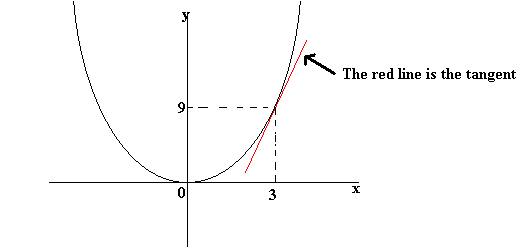
\includegraphics[width=\textwidth]{gradient}
		\end{column}
	\end{columns}
	\begin{itemize}
		\pause\item Equivalent to the \textbf{gradient} of a graph, $\dfrac{\text{change in } y}{\text{change in } x}$		
		\pause\item For moving objects:
		\begin{itemize}
			\pause\item \textbf{Velocity} is the derivative of \textbf{displacement}
			\pause\item \textbf{Acceleration} is the derivative of \textbf{velocity}
			\pause\item NB \textbf{speed} is the \textbf{magnitude} of velocity
		\end{itemize}
	\end{itemize}
\end{frame}

\begin{frame}{Calculus: integration}
	\begin{itemize}
		\pause\item The opposite of differentiation: $x$ is the \textbf{integral} of $\dfrac{dx}{dt}$
		\pause\item We are interested in \textbf{numerical integration}, i.e. by computer calculation
		\pause\item \textbf{Euler method}: given $x$ and $\frac{dx}{dt}$ at time $t$, we can \textbf{estimate} the value of $x$ at time $t+h$:
	\end{itemize}
	\begin{columns}
		\begin{column}{0.58\textwidth}
			\pause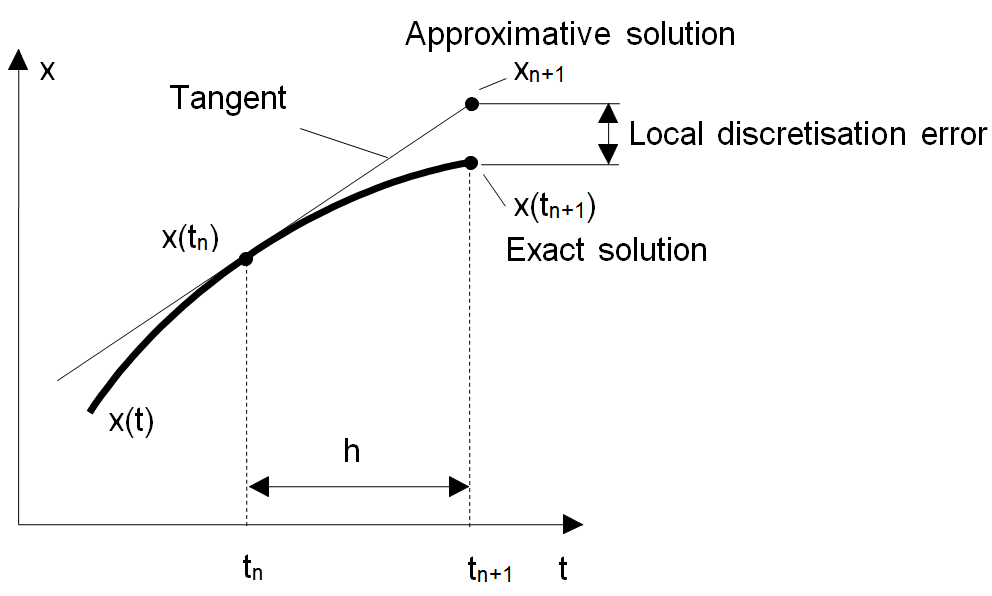
\includegraphics[width=\textwidth]{euler_method}
		\end{column}
		\begin{column}{0.4\textwidth}
			\pause $$ x(t+h) \approx x(t) + h \times \frac{dx}{dt}(t) $$
		\end{column}
	\end{columns}
\end{frame}

\begin{frame}{Basic simulation loop}
	\begin{itemize}
		\pause\item For each object, store its position $\boldsymbol{x}$ and velocity $\boldsymbol{v}$
		\pause\item On each time step $\Delta{t}$:
		\begin{itemize}
			\pause\item Find the new position using numerical integration, $\boldsymbol{x}' = \boldsymbol{x} + $$\boldsymbol{v}\Delta{t}$
			\pause\item Calculate the forces acting on the object, and thus the acceleration $\boldsymbol{a}$ from Newton's second law, $\boldsymbol{F} = m\boldsymbol{a}$
			\pause\item Find the new velocity using numerical integration, $\boldsymbol{v}' = \boldsymbol{v} + $$\boldsymbol{a}\Delta{t}$
		\end{itemize}
	\end{itemize}
\end{frame}

\begin{frame}{Newton's Laws of Motion}
	\begin{center}
		\pause An object remains at rest or moves at constant velocity unless acted upon by an external force
		
		\vspace{2ex}
		
		\pause $\boldsymbol{F} = m\boldsymbol{a}$: The sum of forces acting upon an object is equal to its mass multiplied by its acceleration
		
		\vspace{2ex}
		
		\pause When one body exerts a force on another, the second body exerts an equal and opposite force on the first
	\end{center}
\end{frame}

\begin{frame}{Basic collision response}
	\begin{columns}
		\begin{column}{0.4\textwidth}
			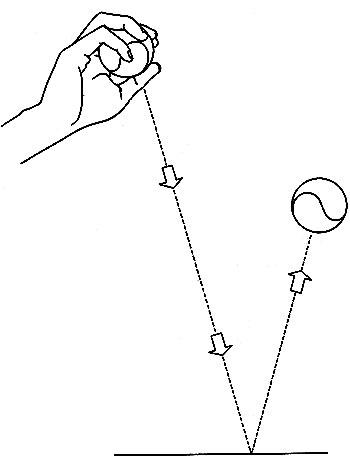
\includegraphics[width=\textwidth]{bounce_reflection}
		\end{column}
		\begin{column}{0.58\textwidth}
			\begin{itemize}
				\pause\item For an \textbf{elastic collision}, the component of velocity parallel to the \textbf{surface normal}
					is \textbf{reversed}
				\pause\item E.g.\ if the surface is the $xz$ plane, flip the $y$ component
				\pause\item For an \textbf{inelastic collision}, some velocity is lost
				\pause\item Flip the $y$ component and multiply it by something between $0$ and $1$
			\end{itemize}
		\end{column}
	\end{columns}
\end{frame}

